\question \textbf{Types of Markov Chains}
\begin{enumerate}[label=(\alph*)]
\item Draw a Markov Chain that is reducible.
\begin{solution}[1.75cm]
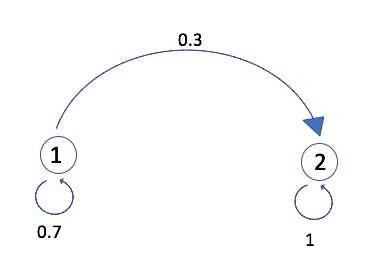
\includegraphics[width=6cm]{reducible.png}
\end{solution}
\item Draw a periodic Markov Chain (note that when we talk about periodicity, we imply that the Markov chain is reducible). Does it have an invariant distribution? Does it always converge to this invariant distribution? Does the invariant distribution represent the average amount of time spent in each state in this chain? 
\begin{solution}[1.75cm]
For the following example, we see that this chain is periodic because in order to get back to a state, you must travel some multiple of 2 steps. For these types of Markov chains, it \textbf{does not always converge} to the invariant distribution. Clearly, in this case the invariant distribution is $\pi = [0.5 0.5]$. However, if we start with the distribuion $\pi_0 = [1 0]$, this distribution will never converge to $\pi$. The invariant distribution \textbf{does represent the average amount of time spent in each state}, because this chain is finite and irreducible. 
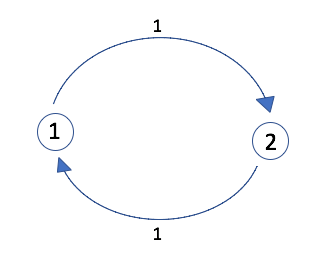
\includegraphics[width=6cm]{periodic.png}
\end{solution}
\item Draw an aperiodic Markov Chain. Does it have an invariant distribution? Does it converge to this
invariant distribution? Does the invariant distribution represent the average amount of time spent in each state in this chain? 
\begin{solution}[2cm]
For these types of Markov chains, it \textbf{always} to the invariant distribution. The invariant distribution \textbf{does represent the average amount of time spent in each state}, because this chain is finite and irreducible. \\
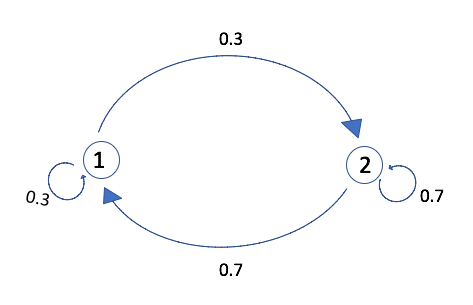
\includegraphics[width=6cm]{aperiodic.png}
\end{solution}
\end{enumerate}